% \subfile{sections/introduction_02}% Opening Context
The rise of autonomous systems is transforming numerous industries, and the maritime sector is no exception. \Acp{USV} have the potential to improve safety and operational efficiency by performing the dull, dirty, and dangerous tasks traditionally done by humans.
Their performance depends on environmental situational awareness, which refers to the system’s ability to perceive relevant features of the surrounding environment. 
Real-time object detection and classification provide the perceptual basis for this capability and are essential for safe navigation and decision making in complex maritime environments.

% Problem Background
Although the automotive industry has achieved significant progress in autonomous perception, comparable advances for maritime platforms remain limited. 
A review of recent literature reveals that studies on autonomous ground vehicles outnumber maritime autonomy publications by nearly one order of magnitude, with a similar disparity observed in object detection research. \textcolor{red}{(cite)}
While some perception strategies from automotive systems can be adapted, the maritime domain introduces fundamentally different challenges. 
Marine environments are unstructured and dynamic, with object densities ranging from sparse to highly dense, particularly in littoral and harbor zones where \acp{USV} frequently operate.

Autonomous maritime systems require high-fidelity sensing to perceive and interact with their immediate operational environment.
Objects must be accurately located and identified so that the \ac{USV} can make informed operational decisions and ensure safe navigation.
Traditional marine radar lacks the spatial resolution needed at these short ranges; instead, uncrewed perception depends primarily on optical and \ac{LiDAR} sensors. \textcolor{red}{(cite)}
Both modalities, however, face significant challenges in dynamic marine conditions.
Visual-spectrum cameras capture rich color and texture information, which is essential for recognizing navigational aids and classifying many objects; however, their performance degrades under conditions such as specular reflections, atmospheric haze, fog, or variable illumination.
Furthermore, camera imagery inherently lacks spatial depth unless supported by additional sensing or estimation methods.
Conversely, \ac{LiDAR} provides precise three-dimensional measurements but lacks the spectral detail required to interpret color-coded or visually distinctive targets.
%%%%%%%%%%%%%%%%%%%%%%%% MRG: Consider making reference to environment with manned/unmanned systems (as this drives the need to interpret colors and the organization that defines navigation aid marker shapes and colors.
These complementary limitations motivate sensor fusion between visual cameras and \ac{LiDAR} scanning to achieve both spatial accuracy and spectral awareness.\textcolor{red}{(cite)}
Real-time fusion is particularly crucial for embedded maritime platforms, where operational demands are high and computational resources are limited.
Efficient fusion frameworks enable low-latency, high-accuracy perception, making them suitable for edge systems that may be constrained by size, weight, and power (SWaP), and better support mission profiles that demand precise and reliable situational awareness, including navigation of littoral zones, search and rescue operations, and defense missions.

\begin{figure}[htpb]
\centering
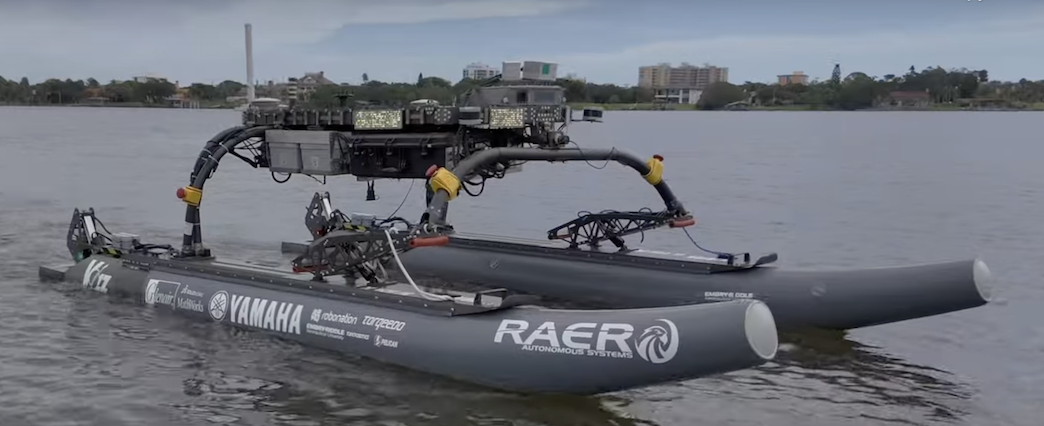
\includegraphics[width=0.9\textwidth]{Images/Minion.png}
\caption{\ac{ERAU}'s research vessel Minion.}
\label{fig:minion}
\end{figure}

\section{Problem Statement}
The central problem addressed by this dissertation is the lack of quantitative, empirical evidence comparing the performance of \ac{LiDAR} and vision-based object detection systems in maritime environments, and the absence of validated real-time fusion strategies that improve detection accuracy beyond single-modality approaches while operating within the computational limits of embedded \ac{USV} platforms.

% Knowledge Gap
% Although research in maritime autonomy continues to expand, several critical gaps persist.  
% First, while many studies have demonstrated the success of vision or \ac{LiDAR}-based detection individually, few provide direct, quantitative comparisons of performance across modalities using identical object classes and conditions.  
% % \textcolor{blue}{Second, the training data requirements and computational efficiency of different sensing modalities have not been systematically characterized, hindering optimal sensor selection for resource-limited platforms. 
% Second, although sensor fusion is widely recognized as advantageous, the tradeoff between the accuracy gains of late fusion and its computational overhead remains poorly quantified for real-time \ac{USV} applications.  
% Finally, reproducible procedures for spatial calibration and temporal synchronization in multi-sensor maritime platforms are inconsistently documented, limiting experimental repeatability and validation.  
% Addressing these gaps requires controlled, empirical evaluation of single- and multi-sensor perception systems using a unified testing framework.
Researchers in maritime perception have primarily focused on vision and \ac{LiDAR} modalities individually, often relying on heterogeneous datasets and differing evaluation protocols. 
Consequently, few studies conduct rigorous quantitative comparisons of identical object classes. \textcolor{red}{(cite)}
Although many propose late fusion to enhance detection robustness, \textcolor{red}{(cite)} few studies consistently or comprehensively characterize the computational cost of fusion in real-time \ac{USV} deployments \textcolor{red}{(cite)}.
Additionally, reports on spatial calibration and temporal synchronization\textcolor{red}{(cite)}, which are required by such fusion techniques, vary widely in scope and detail, undermining reproducibility and complicating cross-study comparisons \textcolor{red}{(cite)}.
This work presents a unified experimental framework for the systematic evaluation of individual detection modalities and introduces a late-fusion approach, along with reproducible procedures for sensor synchronization.

\section{Research Objectives}
Within the domain of surface-level maritime perception under daylight and near-optimal conditions, this research will ultimately show:
% 1. Compare real-time performance of lidar and vision methods in dynamic maritime environment.
% 2. Effective calibration techniques
% 3. Feature analysis for LiDAR-based classification
% 4. Introduction of a Kalman Filter for bounding box object detections
%%%%%%%%%%%%%%%%%%%%%%%% MRG: Your research objectives have 2 verbs.  While minor, I believe bast practice is to have 1.  Check with what was agreed upon by the committee though.
\begin{enumerate}
    \item Characterize the performance differential between vision-based and LiDAR-based object detection systems through quantitative analysis of detection accuracy and computational efficiency.
    \item Develop spatial and temporal calibration techniques for synchronizing asynchronous camera and LiDAR data streams.
    \item Analyze the features extracted for LiDAR-based object classification for their discriminative value and redundancy.
    \item Implement a method that fuses decision-level information from the vision and LiDAR-based detection methods to demonstrate performance improvements over single-mode approaches.
\end{enumerate}

% \begin{enumerate}
%     \item Develop and validate sensor calibration and time-synchronization frameworks for \ac{LiDAR}–camera fusion that:
%     \begin{enumerate}
%         \item Achieve sub-pixel spatial calibration accuracy for point cloud projection, and
%         \item Maintain temporal synchronization with less than 150~ms latency.
%     \end{enumerate}

%     \item Quantify and compare the independent performance of vision- and \ac{LiDAR}-based perception by:
%     \begin{enumerate}
%         \item Determining training data requirements for accurate classification across modalities,
%         \item Evaluating detection and classification performance across representative maritime object classes that vary in geometry and visual characteristics, and
%         \item Identifying the complementary strengths of each modality for integration into fusion architectures.
%     \end{enumerate}

%     \item Implement and evaluate a real-time late-fusion strategy for maritime \ac{USV} applications by:
%     \begin{enumerate}
%         \item Designing and benchmarking a prototype late-fusion framework,
%         \item Comparing computational load and end-to-end latency across detection methods, and
%         \item Establishing quantitative benchmarks to guide future fusion research in maritime perception.
%     \end{enumerate}
% \end{enumerate}

\section{Methodological Overview}
To accomplish these objectives, a modular perception system was developed and deployed on \acposs{ERAU} \ac{USV} research platform, \textit{Minion}.
The system integrates multiple cameras and \ac{LiDAR} sensors with validated spatial and temporal calibration procedures.
%%%%%% MRG: Are the validated calibration procedures referenced here the ones that you developed as part of this research?  As written, it's a bit unclear if it's referring to the work you did here or pre-existing calibration procedures (single modality?)
A comprehensive dataset was collected during the 2024 Maritime RobotX Challenge and dedicated training missions, focusing on six classes of maritime objects.
%%%%%%% MRG:  It would be helpful to provide high-level details about the data collection environments (open water, rivers/lakes, shoreline, etc.)
Data were collected in both open water and controlled marine environments, with most observations acquired under favorable conditions. 
This approach ensured the safety of \ac{ERAU} team members assisting with Minion’s deployment and provided consistency within the dataset. 
These controlled conditions also allow for a clear assessment of baseline system performance. 
More challenging environments, including nighttime operations, fog, rain, and rough seas, are beyond the scope of this work and are identified as important directions for future research.
% \textcolor{blue}{A confidence-weighted late-fusion scheme integrates outputs from both modalities.}
All data are recorded and analyzed within the \ac{ROS} Noetic framework to ensure consistent timing and reproducible evaluation across modalities and fusion configurations.

%%%%%% Coyle: You should note that this study is not meant to point out obvious differences in performance such as the inability for imagery to perform at night
It is important to note that this study is not intended to highlight self-evident differences in performance, such as the limitations of vision-based detection while operating at night, or to evaluate every available detection method.
Instead, the aim is to provide a consistent comparison under controlled conditions between two real-time detection implementations on the Minion platform: vision-based detection using a fine-tuned YOLOv8~\cite{redmon2016} model and LiDAR-based detection using Grid-Based Clustering and Convex Hull Extraction (GB-CACHE)~\cite{coyleE}.
YOLOv8 was selected due to its status as a leading and widely adopted deep learning detection algorithm. 
%%%%%%% MRG: consider omitting the highlighted lines and instead focus on what you selected (GB-CACHE):
A deterministic method for LiDAR detection was selected for two reasons. 
First, comparing two neural network-based approaches would not provide a meaningful comparison between visual and LiDAR sensing modalities. 
Second, it is difficult to enforce strict rules governing system behavior when using neural network methods. 
This becomes a liability when performing high-stakes or other operational tasks that require consistent, predictable behavior.
Deterministic methods, by contrast, operate according to explicitly defined rules by design, making their investigation highly relevant to the situational awareness of uncrewed vessels.
%%%%%%% end MRG
% GB-CACHE was therefore selected as the deterministic method for LiDAR detection. 
This method has demonstrated its capability for real-time use on Minion, and its geometric, rules-based approach makes it both transparent and reproducible. 
These characteristics position GB-CACHE as well-suited to the sensing requirements of uncrewed maritime systems, as well as a strong deterministic counterpart to the neural network-based YOLO method for vision.




\section{Research Impact}
This research makes four principal contributions to the field of maritime autonomy:

\begin{enumerate}
    \item Quantitative Characterization of Real-Time Single-Modality Performance Baselines for USVs
    \item Development and Validation of High-Fidelity Spatiotemporal Sensor Alignment Procedures for Dynamic Platforms.
    \item Information-Theoretic Feature Optimization for Deterministic LiDAR Classification
    % \item \textcolor{blue}{Demonstration and validation of a real-time late-fusion framework that achieves measurable improvements in detection accuracy over the individual sensing-mode detection methods.}
    \item Validation of a Static Kalman Filter for Variance-Weighted Late Fusion to Refine Object Localization.
\end{enumerate}

% These findings directly support \ac{DoN} applications such as autonomous harbor navigation, mine countermeasures, and persistent surveillance. They also inform the development of commercial \ac{USV} systems for environmental monitoring, offshore infrastructure inspection, and autonomous logistics.

% Scope and Limitations
% This study investigates sensor fusion for detecting and classifying marine objects using \ac{LiDAR} and \ac{HDR} camera data collected under daylight and clear-weather conditions. 
The six primary object classes examined in this study include navigational markers and small to mid-sized vessels, each presenting distinct detection challenges. 
%%%%%%%%%% MRG: Consider listing them here.
Tall cylindrical and round navigational markers and buoys exhibit regular geometry favorable to \ac{LiDAR}-based methods, yet encode essential color cues detectable only by cameras. 
Conversely, small watercraft such as flat-bottomed Jon boats and sailboats exhibit variable shapes and appearances that challenge both sensing modalities.

%%%%%%%%%%%% MRG: you talk about study limitations earlier.  Consider grouping these together.

% Data were collected under favorable conditions, specifically in controlled marine environments and open-water scenarios, to ensure the safety of the ERAU team members and for consistency within the dataset. 
% Limiting the study to these conditions allows for a clear assessment of baseline performance. 
% More challenging environments, such as nighttime, fog, rain, and rough seas, are outside the present scope and are acknowledged as areas for future research.

\section{Dissertation Structure}
The remainder of this dissertation is organized as follows.  
Chapter~\ref{litReview} reviews the related literature and research in maritime object detection and sensor fusion. 
Chapter~\ref{sensing_platform} details the sensing platform architecture and hardware integration, methodologies and results for sensor calibration, and a summary of the collected data.  
Chapter~\ref{realtime_object_detection} presents the object detection methods used for visual, LiDAR-based, and late-fusion object detection methods along with their independent detection results and performance evaluation.
Chapter~\ref{chapter_conclusions} provides a discussion comparing the results of YOLO and GB-CACHE, as well as the late-fusion approach to single-mode detection.
Finally, Chapter~\ref{chap:recommendations} concludes with a summary of findings and recommendations for future research.
% \textcolor{blue}{(Add?) Finally, additional figures, tables, and calibration data appear in appendices....}